% Chapter 1

\chapter{Introducción general} % Main chapter title

\label{Chapter1} % For referencing the chapter elsewhere, use \ref{Chapter1} 
\label{IntroGeneral}

%----------------------------------------------------------------------------------------

% Define some commands to keep the formatting separated from the content 
\newcommand{\keyword}[1]{\textbf{#1}}
\newcommand{\tabhead}[1]{\textbf{#1}}
\newcommand{\code}[1]{\texttt{#1}}
\newcommand{\file}[1]{\texttt{\bfseries#1}}
\newcommand{\option}[1]{\texttt{\itshape#1}}
\newcommand{\grados}{$^{\circ}$}

%----------------------------------------------------------------------------------------

%\section{Introducción}

%----------------------------------------------------------------------------------------
En este capítulo se exponen los problemas encontrados con el hardware en el estudio de los sistemas embebidos y la necesidad de un emulador para la placa EDU-CIAA-NXP \citep{EDU-CIAA-NXP}. También se describe el estado actual de algunas soluciones implementadas y una breve descripción de la plataforma propuesta.

\section{Motivación}

Teniendo en cuenta la complejidad en el aprendizaje de programación de sistemas embebidos para los desarrolladores principiantes y, además, siendo el principal problema la interacción con el hardware, se propuso, como parte del proyecto CIAA \citep{CIAA}, una plataforma que emule la placa EDU-CIAA-NXP.

Ahora bien, considerando que para el desarrollo de aplicaciones en sistemas embebidos es necesario tener de antemano la placa de desarrollo y los componentes de hardware para comenzar con el programa y, además, muchas veces un usuario sin experiencia no cuenta o se equivoca en la selección de los dispositivos para comenzar, una alternativa interesante es la utilización de una plataforma de emulación que permita al usuario probar determinados programas rápidamente.

Es decir, de esta manera, los usuarios principiantes podrían enfocarse en desarrollar sus aplicaciones y ejecutar sus pruebas en un sistema virtual dejando para más adelante la implementación en el hardware real.

El valor de tener un emulador podría apreciarse en estas cuatro aplicaciones prácticas:
\begin{itemize}
	\item A nivel docente y de enseñanza en escuelas o academias de formación en programación de sistemas embebidos.
	\item Como herramienta para realizar primeras pruebas.
	\item Como herramienta para evaluar programas que no funcionen como se esperába, ya que se aísla el hardware.
	\item Solución valiosa que permite a los estudiantes con bajos recursos económicos acceder virtualmente a hardware costoso.
\end{itemize}


%----------------------------------------------------------------------------------------

\section{Descripción técnica-conceptual}

Los emuladores son desarrollos de software que modelan de forma precisa el funcionamiento del hardware real, de manera que permiten ejecutar programas dentro de un ambiente que imita su comportamiento \citep{sanchezqemu}. De esta forma el usuario puede simular su código antes de instalarlo en el dispositivo físico.

Por consiguiente, teniendo en cuenta dichas características, el presente trabajo se centró en construir una plataforma de desarrollo con interfaz gráfica que realiza la emulación de la placa EDU-CIAA-NXP dentro de un entorno web. La arquitectura responde a la emulación a nivel de API \citep{API}, para lo cual fue necesario integrar y adaptar las sAPI del proyecto CIAA.

En la figura \ref{fig:EsquemaEmulador} se observa una computadora que debe acceder a la plataforma de emulacion de la placa EDU-CIAA-NXP mediante un navegador web. Entonces, la herramienta imitará las características de hardware e incluso las de software dentro del entorno de programación en la computadora del usuario, todo de manera virtual.

\begin{figure}[ht]
	\centering
	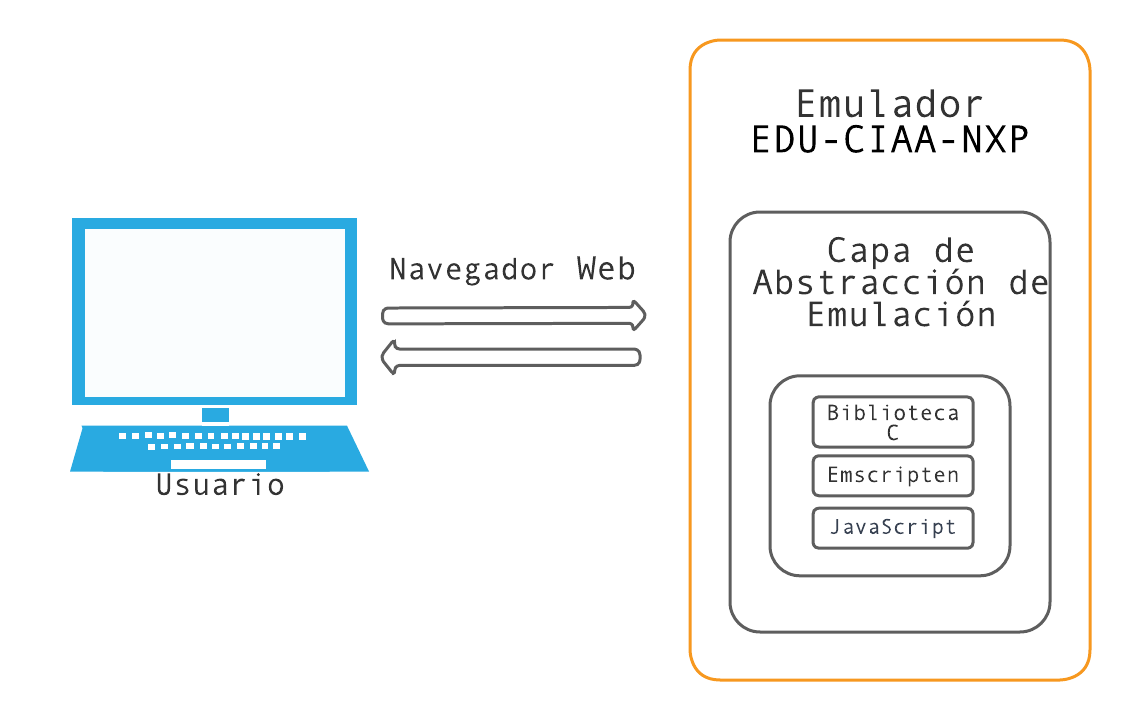
\includegraphics[scale=.60]{./Figures/EsquemaEmulador.png}
	\caption{Esquema Emulador EDU-CIAA-NXP.}
	\label{fig:EsquemaEmulador}
\end{figure}

En otras palabras, con esta herramienta de emulación, una persona que recién comienza tendrá la experiencia de relacionarse con un sistema embebido solamente conectandose mediante internet a la aplicación web en su ordenador, liberando así el camino a los estudiantes primerizos de hacer la interacción con el hardware.
%----------------------------------------------------------------------------------------

\section{Estado del arte}

Hoy en día no existe una herramienta de emulación para la placa EDU-CIAA-NXP. Sin embargo, existe la plataforma de código abierto ViHard \citep{ViHard} que emula dispositivos de hardware en la PC, pero conectada a la placa real a través del puerto USB. 

La plataforma se compone de: un programa de PC con los perifericos virtuales de hardware y un programa de firmware con una biblioteca embebida, que controla y gestiona el funcionamiento del hardware virtual. Ambos programas se comunican con el sistema embebido mediante un puerto USB.

El programa de hardware virtual es una aplicacion de escritorio multiplataforma desarrollada utilizando el framework Electron \citep{Electron}. Por otro lado, la biblioteca embebida fue desarrollada en lenguaje C. 

Por lo tanto, el usuario necesita ejecutar en su PC el programa de periféricos virtuales y contar con la biblioteca en el sistema embebido que controla el hardware virtual. A partir de ahí, procedería al desarrollo de su propio algoritmo y posteriormente realizar las pruebas correspondientes.


La figura \ref{fig:ViHard} muestra el esquema de la plataforma ViHard.

\begin{figure}[ht]
	\centering
	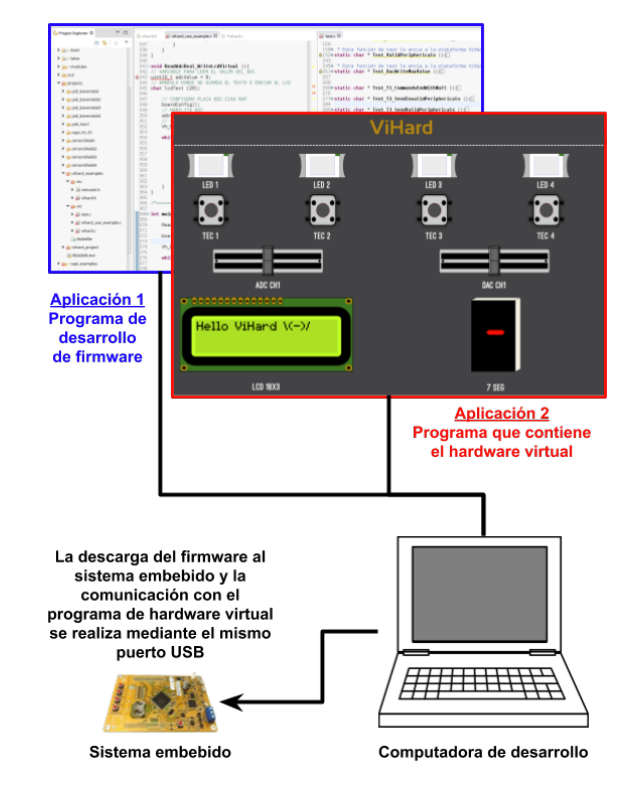
\includegraphics[scale=.40]{./Figures/ViHard.png}
	\caption{Esquema de la plataforma ViHard.\protect\footnotemark}
	\label{fig:ViHard}
\end{figure}

\footnotetext{Imagen tomada de \url{http://laboratorios.fi.uba.ar/lse/tesis/LSE-FIUBA-Trabajo-Final-MSE-Agustin-Bassi-2018.pdf}}

Además, se encontraron dentro de las plataformas educativas muchos simuladores para microntroladores, sobre todo para la placa Arduino \citep{Arduino}. Para el análisis, se seleccionaron algunos de los simuladores más populares que además, implementan funcionalidades relevantes para el presente trabajo. 

UnoArduSim \citep{UnoArduSim} fue desarrollado en la Universidad de Queen \citep{Queensu} por el profesor Stan Simmons. La herramienta simula en la pantalla de la PC la placa Arduino Uno \citep{ArduinoUno} y muchos de los dispositivos de entrada y salida más usados, asimismo, permite la depuración interactiva de funciones o programas completos. Por otro lado, está diseñada específicamente para ejecutarse en el sistema operativo Windows, además, el diseño de la interfaz gráfica no promueve la claridad visual, puesto que hay demasiados objetos en la pantalla y los que existen deberían estar mejor distribuidos. 

En la figura \ref{fig:UnoArduSim} puede observarse la interfaz de la aplicación.
\hfill \break
\hfill \break
\hfill \break
\hfill \break

\begin{figure}[ht]
	\centering
	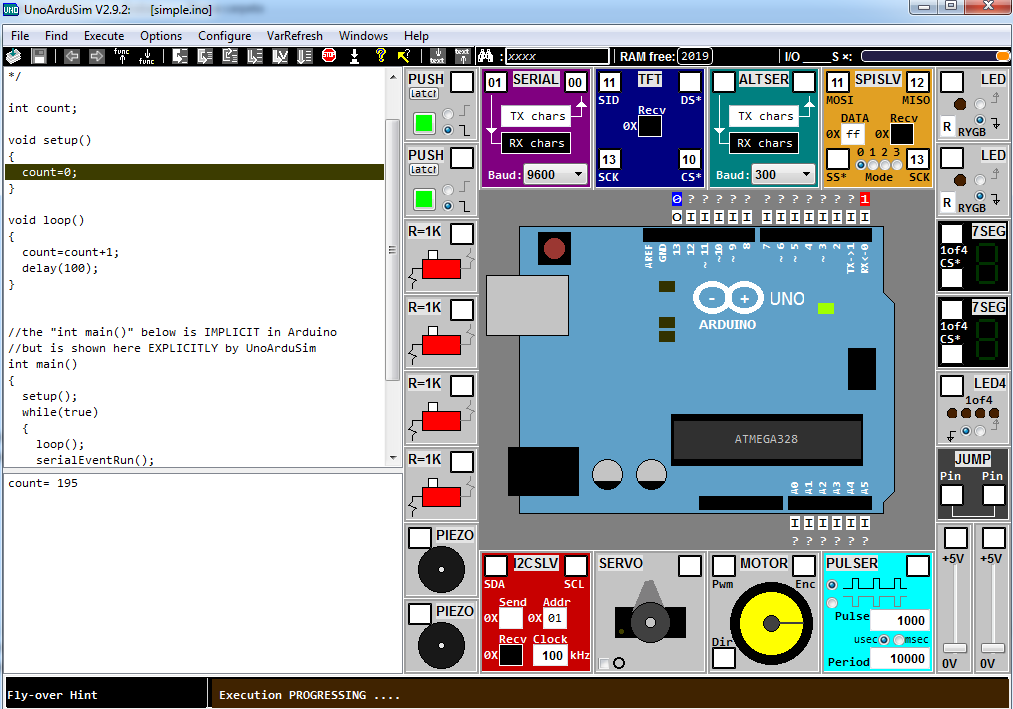
\includegraphics[scale=.33]{./Figures/UnoArduSim.png}
	\caption{Plataforma UnoArduSim.}
	\label{fig:UnoArduSim}
\end{figure}



Virtronics \citep{Virtronics} es uno de los simuladores más completos que hay hoy en día para Arduino \citep{Arduino}, ya que permite simular varios modelos y, además, tiene dos versiones disponibles: una versión paga y otra gratuita, pero con funciones limitadas. 

En la figura \ref{fig:Virtronics} se muestra la plataforma.

\begin{figure}[ht]
	\centering
	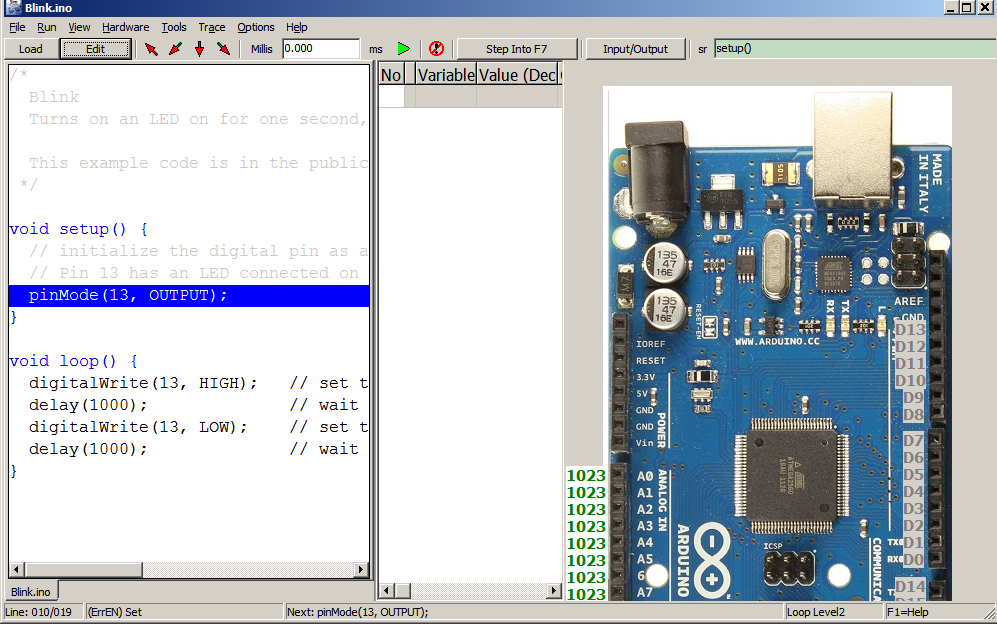
\includegraphics[scale=.35]{./Figures/Virtronics.png}
	\caption{Plataforma Virtronics.}
	\label{fig:Virtronics}
\end{figure}


Tinkercad \citep{Tinkercad} es una plataforma online que permite el acceso desde cualquier navegador web. Fue desarrollado por ingenieros y diseñadores de software de Autodesk \citep{Autodesk} y permite diseños 3D. Adicionalmente, es necesario crear una cuenta  antes de empezar a usar la plataforma, por consiguiente, todos los diseños se guardan en la cuenta creada.

En la figura \ref{fig:Tinkercad} puede observarse la interfaz de usuario.

\begin{figure}[ht]
	\centering
	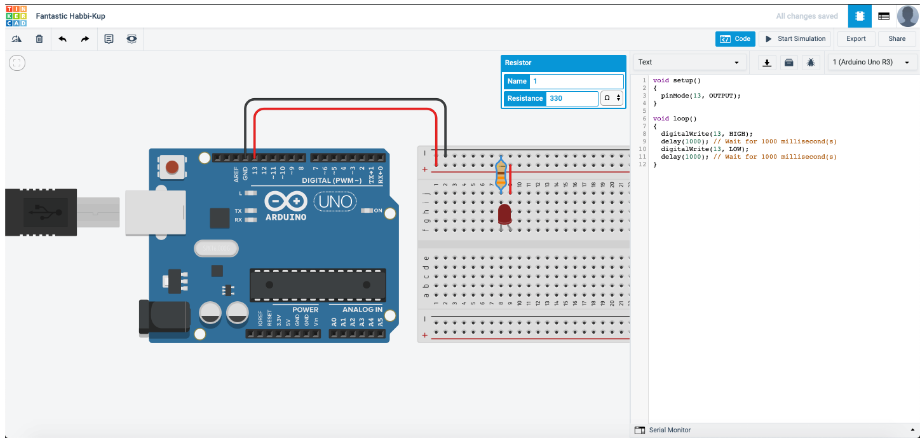
\includegraphics[scale=.42]{./Figures/Tinkercad.png}
	\caption{Plataforma Tinkercad.}
	\label{fig:Tinkercad}
\end{figure}


Mbed Simulator \citep{ArmMbedSim} fue desarrollado por ingenieros de Mbed \citep{ArmMbed} y es parte de Mbed Labs. La plataforma es accesible en línea y se puede utilizar desde cualquier navegador web

En la figura \ref{fig:ArmMbed} puede observarse la plataforma online de Mbed Simulator.


\begin{figure}[ht]
	\centering
	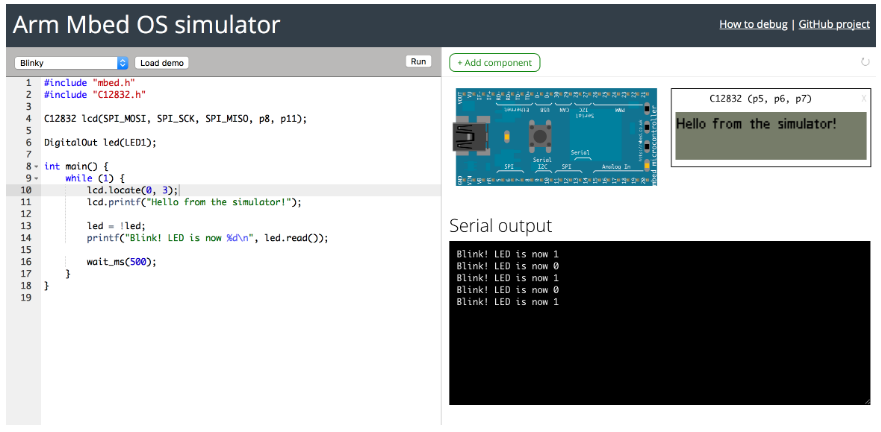
\includegraphics[scale=.44]{./Figures/ArmMbed.png}
	\caption{Plataforma Mbed Simulator.}
	\label{fig:ArmMbed}
\end{figure}

El funcionamiento de este emulador es muy simple. Se puede crear un programa desde cero, o bien, se puede elegir un ejemplo de la lista desplegable y cargar el proyecto desde el botón \textquotedbl Load demo\textquotedbl, luego añadir los componentes necesarios para el programa, como por ejemplo, el display que se observa en la figura \ref{fig:ArmMbed}, donde se pide al usuario indicar a qué pines estará conectado. Es importante mencionar que el programa ya incluye la placa con el microcontrolador precargada. Una vez completo el programa y el ensamblado del hardware, se puede compilar y ejecutar en el emulador usando el botón \textquotedbl Run\textquotedbl.

En la tabla \ref{tab:simuladores} se presenta algunas de las características más importantes que tienen en común estas plataformas y también, algunas de las diferencias encontradas.

\begin{table}[h]
\centering
\caption[Comparación de características de plataformas de simulación]{Comparación de características de plataformas de simulación}
\begin{tabular}{p{0.24\linewidth} p{0.17\linewidth}  p{0.19\linewidth}  p{0.14\linewidth}  p{0.10\linewidth}}
\toprule
\textbf{Característica} 
& \textbf{UnoArduSim}
& \textbf{Virtronics}
& \textbf{Tinkercad}
& \textbf{Mbed}
\\
\midrule
Microcontrolador & Arduino Uno & Varios modelos Arduino & Arduino Uno & Arm\\
Gratuito &    Sí & No & Sí & Sí\\
Aplicación & Escritorio & Escritorio & Web & Web\\
Plataforma & Windows & Windows/Linux & Todas & Todas\\
Código abierto & No & Sí & No & Sí\\
Dispositivos E/S & Sí & Sí & Sí & Sí  \\
Panel de desarrollo & Sí & Sí & Sí & Sí \\
Lenguaje & C & C & C & C/C++\\
Debugging & Sí & Sí & Sí & No\\
Biblioteca ejemplos & Sí & Sí & Sí & Sí\\
\bottomrule
\hline
\end{tabular}
\label{tab:simuladores}
\end{table}


Para realizar el presente trabajo final, se decidió basarse en el proyecto Mbed Simulator debido a las siguientes ventajas significativas:

\begin{itemize}
	\item Comunidad y Soporte: el proyecto tiene una comunidad activa de desarrolladores, que brinda acceso a una amplia base de conocimientos, documentación y soporte. 
	\item Reconocimiento de Marca ARM mbed OS: al basarse en su proyecto simulador, se puede obtener cierto reconocimiento y confianza entre los usuarios.
	\item Código abierto: al tener acceso al código fuente permitió estudiar cómo funciona internamente el proyecto simulador, además, de la libertad de uso y distribución.
	\item Reutilización: ofrece un conjunto sólido de funcionalidades y características ya probadas que agilizó el desarrollo y redujo la probabilidad de introducir errores.
	\item Actualizaciones y Mejoras Continuas: el proyecto Mbed Simulator recibe actualizaciones continuas con las últimas tecnologías que permite mantener el emulador para la placa EDU-CIAA-NXP actualizado.
	
\end{itemize}



%----------------------------------------------------------------------------------------

\section{Propósito y Alcance}

\subsection{Propósito}

El propósito de este trabajo fue desarrollar una herramienta educativa que brinda un entorno virtual para la placa EDU-CIAA-NXP, permitiendo al usuario seleccionar e interactuar con diferentes tipos de dispositivos virtuales de entrada/salida. Este desarrollo permite al usuario cargar,
ejecutar, editar y corregir sus programas escritos en lenguaje C, pudiendo monitorizar gráficamente en la pantalla del ordenador la placa EDU-CIAA-NXP y muchos de los dispositivos de entrada y salida más usuales, todo de manera virtual, sin necesidad de disponer de ningún dispositivo de hardware.

\subsection{Alcance}

Para la realización de este trabajo se realizó una primera versión de la herramienta para ser usada con la placa EDU-CIAA-NXP.

En el presente trabajo se incluyen los siguientes aspectos:

\begin{enumerate}
	\item Desarrollo de aplicación para emular el hardware en PC.
	\item Desarrollo de programas de ejemplo para ser usados dentro de la aplicación.
	\item Documentación de referencia.
\end{enumerate}

El presente proyecto NO incluye los siguientes aspectos:

\begin{enumerate}
	\item Desarrollo de la aplicación para emular otras placas que no sea EDU-CIAA-NXP.
\end{enumerate}